\chapter{信号的采样与重建}

\begin{introduction}
  \item 信号采样与重建流程
  \item 基于\textit{Simulink}的信号采样与重建仿真
  \item 基于\textit{MATLAB}的信号采样频谱绘制
\end{introduction}

\section{实验背景与目的}
  

本实验旨在探讨信号采样过程中的频谱变化,分析采样是否会导致信息丢失,并评估采样序列能否充分代表原始信号,同时研究如何实现不失真的信号还原。通过对奈奎斯特采样定理的理解与验证,深入分析采样频率与信号最高频率之间的关系,并研究当采样定理不满足时可能出现的频谱混叠现象及其影响。此外,实验将研究离散时间信号的采样(抽取)、插值及采样率转换的基本原理与实现方法,并观察这些操作在时域和频域中的特性变化。针对信号采样与重建过程中的关键环节,本实验还将介绍模拟低通滤波器的指标特性,包括抗混叠滤波器和平滑滤波器的作用,并探讨其设计要求及实际应用中的挑战。最终,通过 MATLAB 和 Simulink 搭建实验平台,进行信号采样与重建实验,验证理论知识,分析实验结果,并通过解决实验过程中遇到的问题,提高实践操作和数据分析能力。

\section{实验原理}

\subsection{信号采样基础}
信号采样是指对连续时间信号 $x(t)$ 按固定采样周期 $T$ 进行取值,得到离散时间信号 $x[n]$,其中:
\begin{equation}
    x[n] = x(nT), \quad n \in \mathbb{Z}.
\end{equation}
实际采样系统一般包括采样保持器(Sample-and-Hold)和模数转换器(A/D Converter)。采样保持器用于保持瞬时幅度,而 A/D 转换器完成模拟信号与数字信号的转换。

在理想采样条件下,采样过程可看作原始信号与冲激函数序列 $\delta_T (t)$ 相乘:
\begin{equation}
    x_s (t) = x(t) \sum_{n=-\infty}^{\infty} \delta (t - nT).
\end{equation}
其中,$\delta (t)$ 为单位冲激函数。当脉冲宽度 $\tau$ 远小于采样周期 $T$ 时,实际采样接近理想采样。

\subsection{采样信号的频谱特性}
在频域中,采样的本质是对原始信号的频谱 $X(\Omega)$ 进行周期延拓,采样信号的频谱表示为:
\begin{equation}
    X_s(\Omega) = \frac{1}{T} \sum_{k=-\infty}^{\infty} X\left(\Omega - k\Omega_s\right),
\end{equation}
其中 $\Omega_s = \frac{1}{T}$ 是采样频率,$\Omega$ 为连续频率变量。由此可见,采样信号的频谱是原始信号频谱的周期重复。

根据奈奎斯特采样定理,若信号的最高频率 $\Omega_{\max}$ 满足:
\begin{equation}
    \Omega_s \geq 2\Omega_{\max},
\end{equation}
则可以通过带宽为 $\Omega_s/2$ 的理想低通滤波器完美重建原信号。当 $\Omega_{\max} > \Omega_s/2$ 时,会发生\textbf{频谱混叠}(aliasing),即高频分量叠加到低频范围,导致信息损失。为了避免混叠,实际应用中通常选择更高的采样频率,并在采样前使用抗混叠低通滤波器。


\subsection{模拟低通滤波器特性}
抗混叠滤波器用于在采样前抑制高于 $\Omega_s/2$ 的频率成分,以防止频谱混叠。然而,理想低通滤波器的矩形频率响应在实际中无法实现,因此采样频率越低,对抗混叠滤波器的要求越高。

在信号重建过程中,\textbf{平滑滤波器} 主要用于去除 D/A 转换后信号中的高频成分。对于理想的平滑滤波器,其频率响应呈指数衰减,在 $\Omega = k\Omega_s$ 处取零。

\subsection{带通信号的采样}
对于带通信号,其频谱分布于 $\left[\Omega_1, \Omega_2\right]$,其中 $\Omega_2 - \Omega_1 = \Delta\Omega$ 为信号带宽。若 $\Omega_2$ 是带宽的整数倍,则可以选择欠采样方式,此时采样频率 $\Omega_s$为
\begin{equation}
    \Omega_s = 2\Delta\Omega.
\end{equation}
欠采样后,由于低频有大量带宽没有传输信号,若满足适当的带通滤波条件,仍可恢复原信号。并且如果 $\Omega_2$ 不是 $\Delta\Omega$ 的整数倍,则可通过频带扩展调整信号频谱以满足采样条件。

\subsection{离散时间信号的处理}
\begin{definition}[离散时间信号的抽取]
  抽取(Decimation) 指对信号进行降采样,即每隔 $M$ 个采样点保留一个:
\begin{equation}
    x_d[n] = x[Mn].
\end{equation}
\end{definition}

由于采样频率降低了M倍,这种信号处理方式还被称为\textbf{M倍降采样}。为了防止混叠,降采样前需使用抗混叠低通滤波器。

\begin{definition}[离散时间信号的插值]
  插值(Interpolation)指对信号进行升采样,即在相邻采样点之间插入 $L-1$ 个零值:
\begin{equation}
    x_i[n] = \begin{cases}
        x[n/L], & n = 0,  L,  2L, \ldots, \\
        0, & \text{其他}.
    \end{cases}
\end{equation}
\end{definition}

插值用于提高采样率,最简单的方法是插零,然后通过数字低通滤波器去除镜像分量。在语音信号处理等专门领域中,插入的值由专用算法指定,以获得更好的重建质量。

将抽取和插值结合起来便是\textbf{采样率转换}(Sample Rate Conversion)技术。它是指采样率按有理数 $L/M$ 进行变换的方法,通常采用先插值$L$ 倍,再抽取$M$倍的方式实现。转换过程中,在升降采样的间隙必须使用合适的低通滤波器来抑制高频成分,以避免失真。值得注意的是,这个滤波器既承担了抗混叠的作用,也起到了平滑滤波的作用。


\section{实验使用软件}
\begin{itemize}
  \item MATLAB 2024b
  \item Simulink 2024b
\end{itemize}

\section{实验内容}

\subsection{基于 Simulink 的信号采样与重建时域仿真}

利用Simulink搭建信号采样与重建仿真系统,验证信号采样与重建的基本原理。在这个实验中,我们使用正弦波通过经过采样后通过一切比雪夫低通滤波器的模型为例,分析各个阶段中信号是如何采样重建的。具体步骤如下:
\begin{itemize}
  \item 搭建实验模型,如图~\ref{fig:model1}~所示。
  \item 设置正弦波的频率为 $f = 1$ kHz,脉冲波的频率为 $f = 5$ kHz,占空比25\%。给定低通滤波器的截止频率为 $f_c = 1.5$ kHz。
  \item 启动仿真,观察\lstinline{Scope}中的波形。
\end{itemize}
\begin{figure}[htbp]
  \centering
  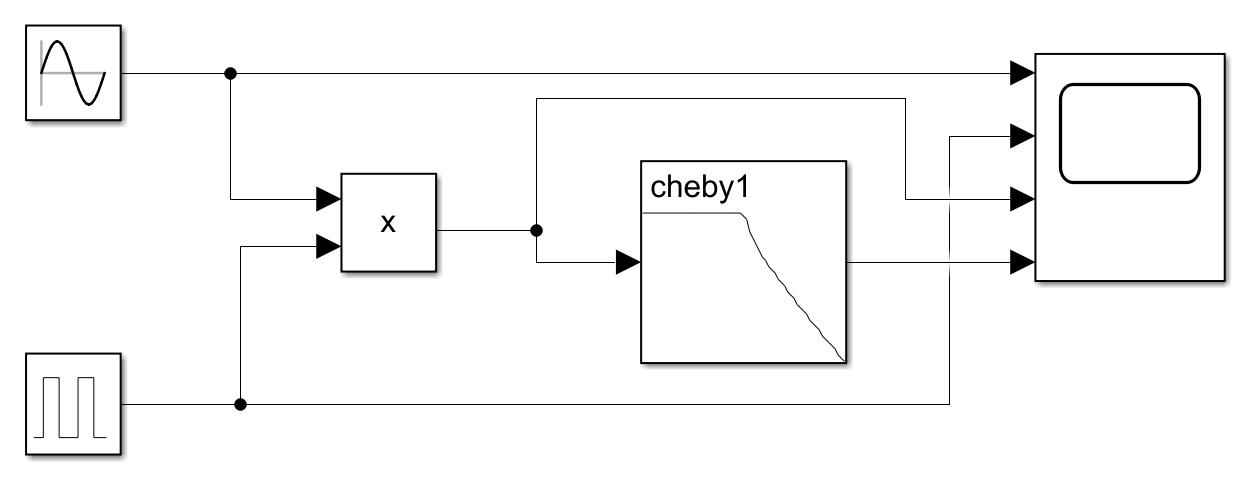
\includegraphics[width=0.5\textwidth]{figure/exp1/model1.png}
  \caption{信号采样与重建仿真模型}
  \label{fig:model1}
\end{figure}

\begin{figure}[htbp]
  \centering
  \subfloat[默认参数下的信号采样重建波形\label{fig:sim1}]{
    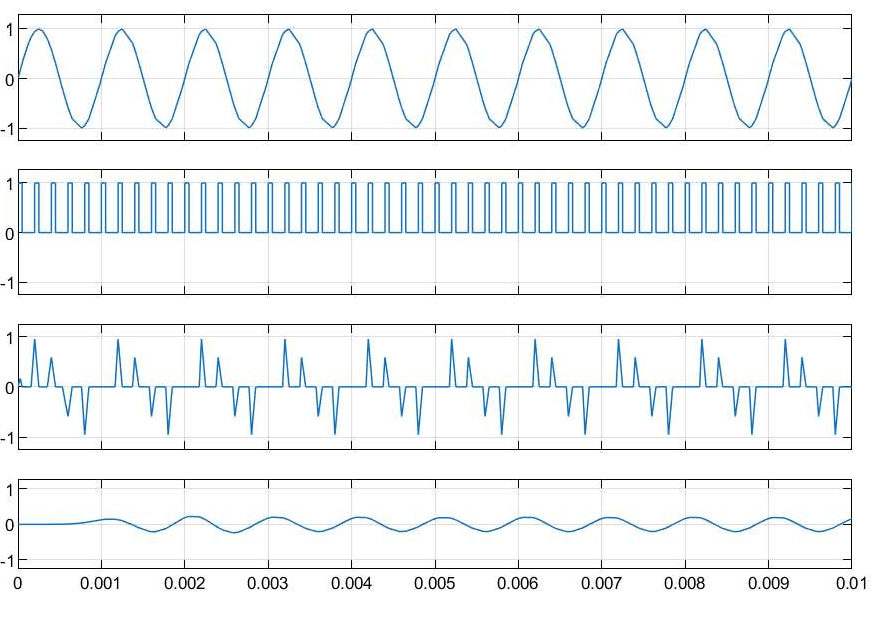
\includegraphics[width=0.45\textwidth]{figure/exp1/sim1.pdf}
  }
  \hfill
  \subfloat[$f_s$=1.5kHz时的采样重建波形\label{fig:sim2}]{
    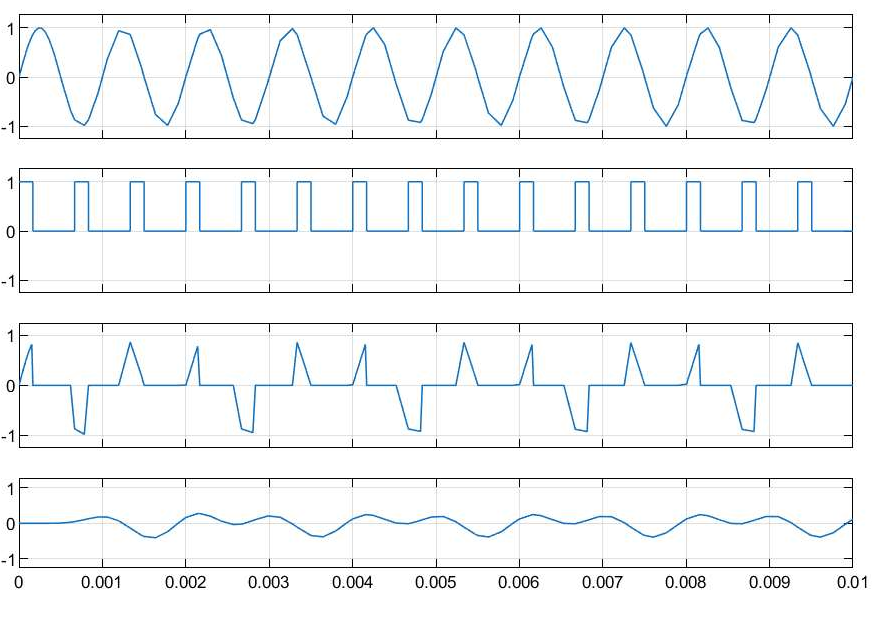
\includegraphics[width=0.45\textwidth]{figure/exp1/sim2.pdf}
  }
  \newline
  \subfloat[低通滤波器截止频率为5kHz时的信号重建\label{fig:sim3}]{
    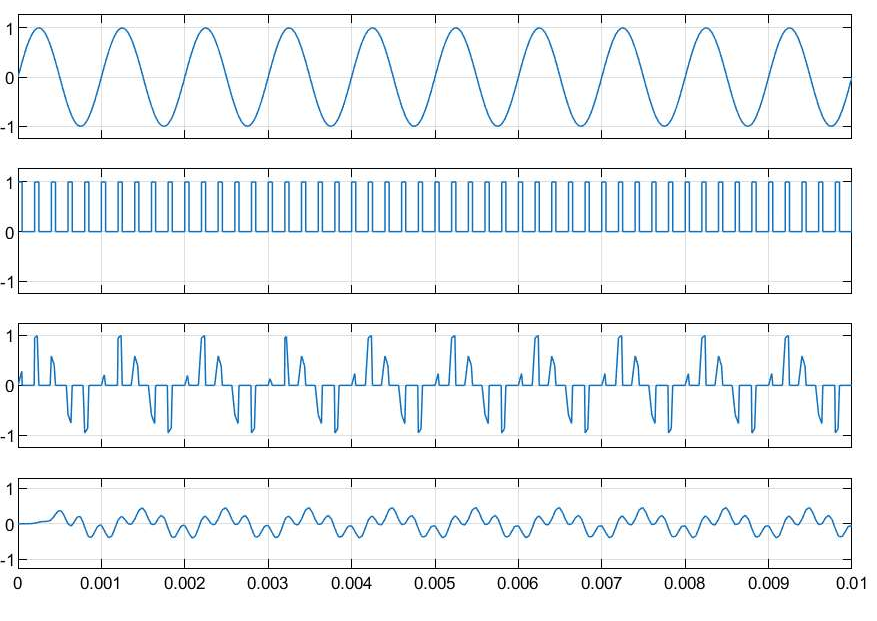
\includegraphics[width=0.45\textwidth]{figure/exp1/sim3.pdf}
  }
  \hfill
  \subfloat[冲激信号占空比50\%时的信号重建\label{fig:sim4}]{
    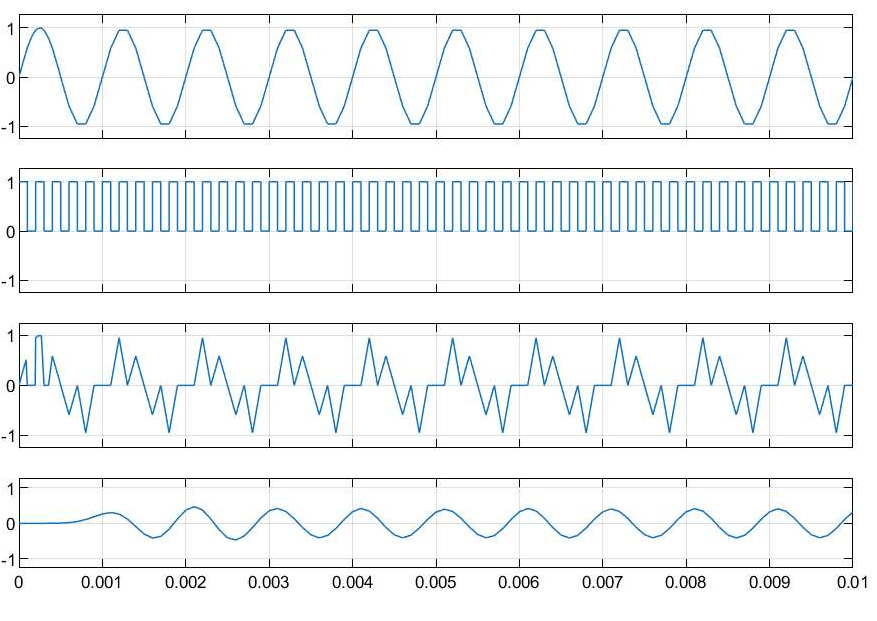
\includegraphics[width=0.45\textwidth]{figure/exp1/sim4.pdf}
  }
  \caption{信号采样与重建时域仿真结果}
  \label{fig:sim}
\end{figure}

默认参数下的仿真结果如图~\ref{fig:sim1}~所示。从上到下的四条波形分别为发射正弦波、采样冲激信号、采样信号和重建信号。可以看到,重建信号的频率与原始信号一致,但幅度有所损失。接下来,为了验证奈奎斯特采样定理,将采样频率降低为1.5kHz,重新进行仿真。仿真结果如图~\ref{fig:sim2}~所示。可以看到,重建信号“叠”在了一起,和原始信号有明显的差异。故认为该采样频率下信号出现了混叠。保持采样频率为5kHz,将低通滤波器的截止频率调整为5kHz,重新进行仿真。仿真结果如图~\ref{fig:sim3}~所示。可以看到,重建信号的频率大体上与原始信号一致,但是波形出现了抖动。这说明,低通滤波器可以滤除高频分量,从而使得重建信号更加平滑。最后,为了验证脉冲信号宽度对重建信号性能的影响,将脉冲信号占空比调至50\%,观察仿真波形如图~\ref{fig:sim4}~所示。可以看到采样信号和重建信号的幅值都变大了,这是由于脉冲信号的占空比增大,使得采样信号的幅值增大。


\subsection{基于Simulink的信号采样仿真}

在进行模型时域波形仿真后,进一步利用Simulink分析信号采样的频谱特性。具体步骤如下:
\begin{itemize}
  \item 搭建实验模型,如图~\ref{fig:model2}~所示。
  \item 设置三个正弦波发生器的频率分别为 $f_1 = 500$ kHz,$f_2 = 4400$ kHz,$f_3 = 5800$ kHz。设置合成波的三种采样频率分别为30MHz,10MHz和3MHz,幅值分别为10,5,1。\footnote{按照课上讲义,这里取了更高的采样频率以免显示不全。}
  \item 启动仿真,观察\lstinline{Scope},\lstinline{Scope1}和\lstinline{Spectrum Analyzer}中的频谱。

\end{itemize}

\begin{figure}[htbp]
  \centering
  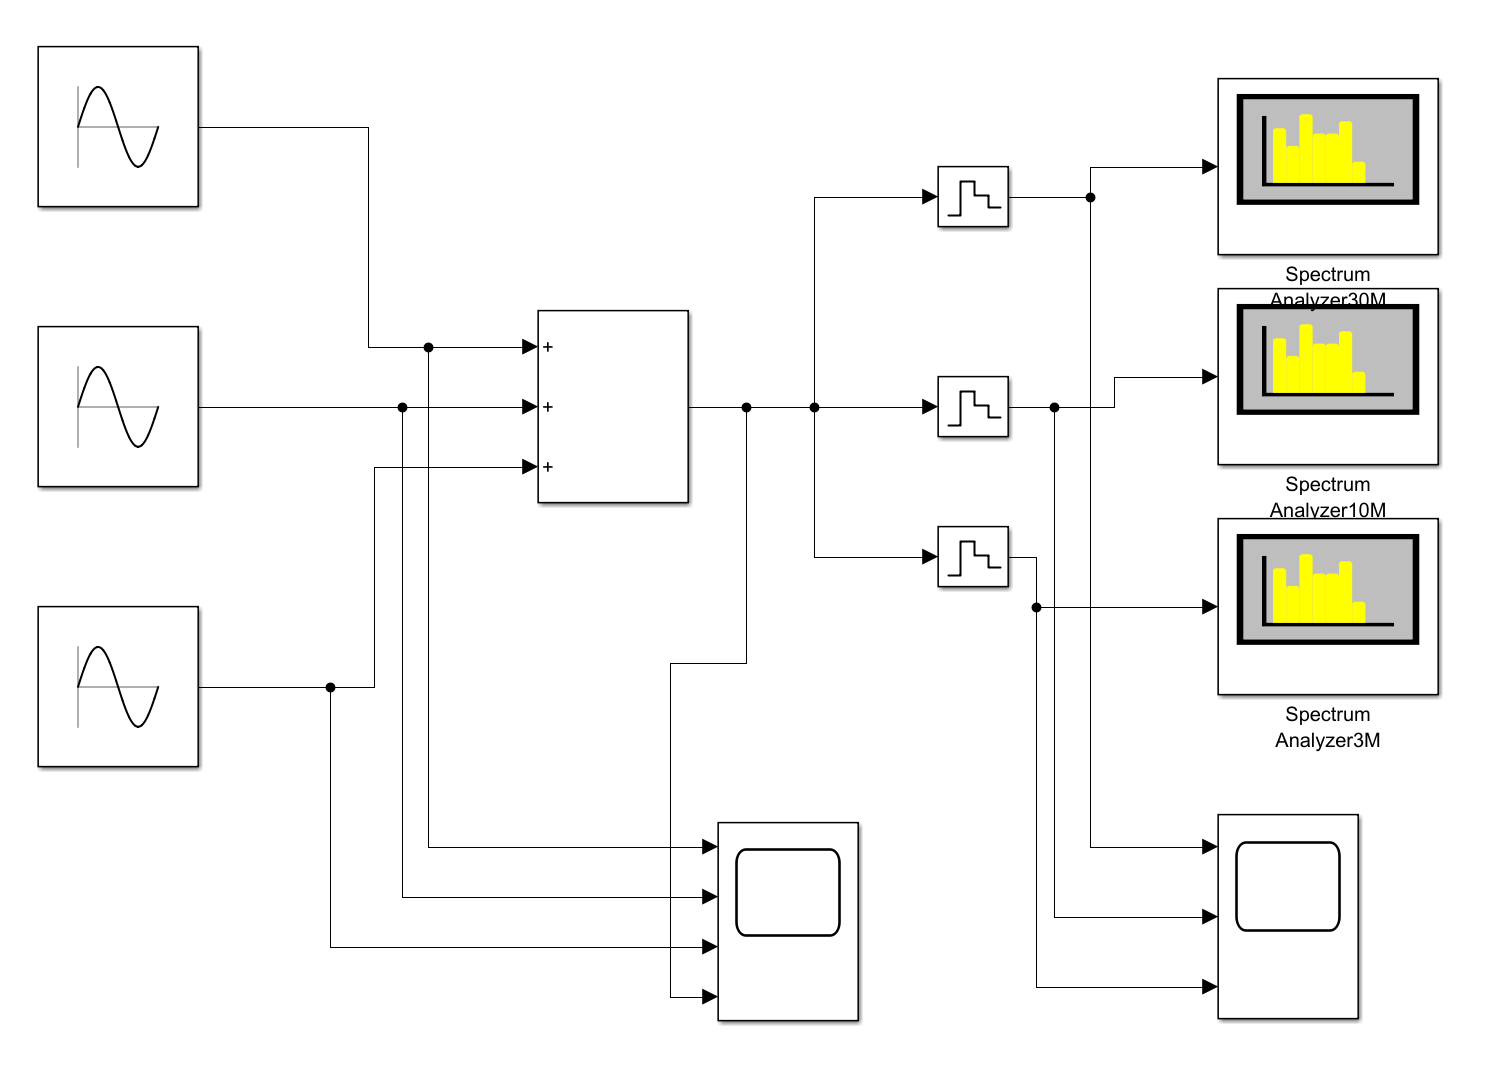
\includegraphics[width=0.65\textwidth]{figure/exp1/model2.png}
  \caption{信号采样与重建频域仿真模型}
  \label{fig:model2}
\end{figure}

启动仿真后,首先观察\lstinline{Scope}的结果,如图~\ref{fig:sim2_1}~所示。使用青蓝色标注第一个频率为$f_1$的正弦波,使用天蓝色标注第二个频率为$f_2$的正弦波,使用黄绿色标注第三个频率为$f_3$的正弦波,并用墨绿色标注通过加法器后的正弦波。可以看到,三个正弦波的频率分别为500kHz,4400kHz和5800kHz。通过加法器的正弦波周期为三个正弦波周期的最小公倍数,因此频率最小。

接下来,观察\lstinline{Scope1}的结果,如图~\ref{fig:sim2_2}所示。使用青蓝色标注采样频率为$f_{s1} = 30$MHz的波形,使用天蓝色标注采样频率为$f_{s2} = 10$MHz的波形,使用黄绿色采样频率为$f_{s3} = 3$MHz的波形。可以看到,加和正弦波的频率通过保持器后保持不变,但变成了阶跃形的波形。采样频率越高,阶跃次数越多,越贴近真波形。

最后,观察\lstinline{Spectrum Analyzer}的结果如图~\ref{fig:spectrum30}~、~\ref{fig:spectrum10}~、~\ref{fig:spectrum3}~所示。观察对称频谱的峰值,可以看到清晰的三根谱线。在前两个图中,信号的峰值出现在预设频率 0.5 MHz、4.4 MHz 和 5.8 MHz 附近,且幅度经过V/dBm的$20\log$计算公式换算后保持一致。三个峰值中,最大值与最小值的差异约为 20 dB,与理论计算结果一致。然而,在采样频率为10MHz的结果中,频率峰值偏离了设定值,这可能是由于该频率分量与FFT采样点不对齐导致的栅栏效应,或者该频率分量出现了泄露。  



\begin{figure}[htbp]
    \centering
    \subfloat[采样前的时域波形\label{fig:sim2_1}]{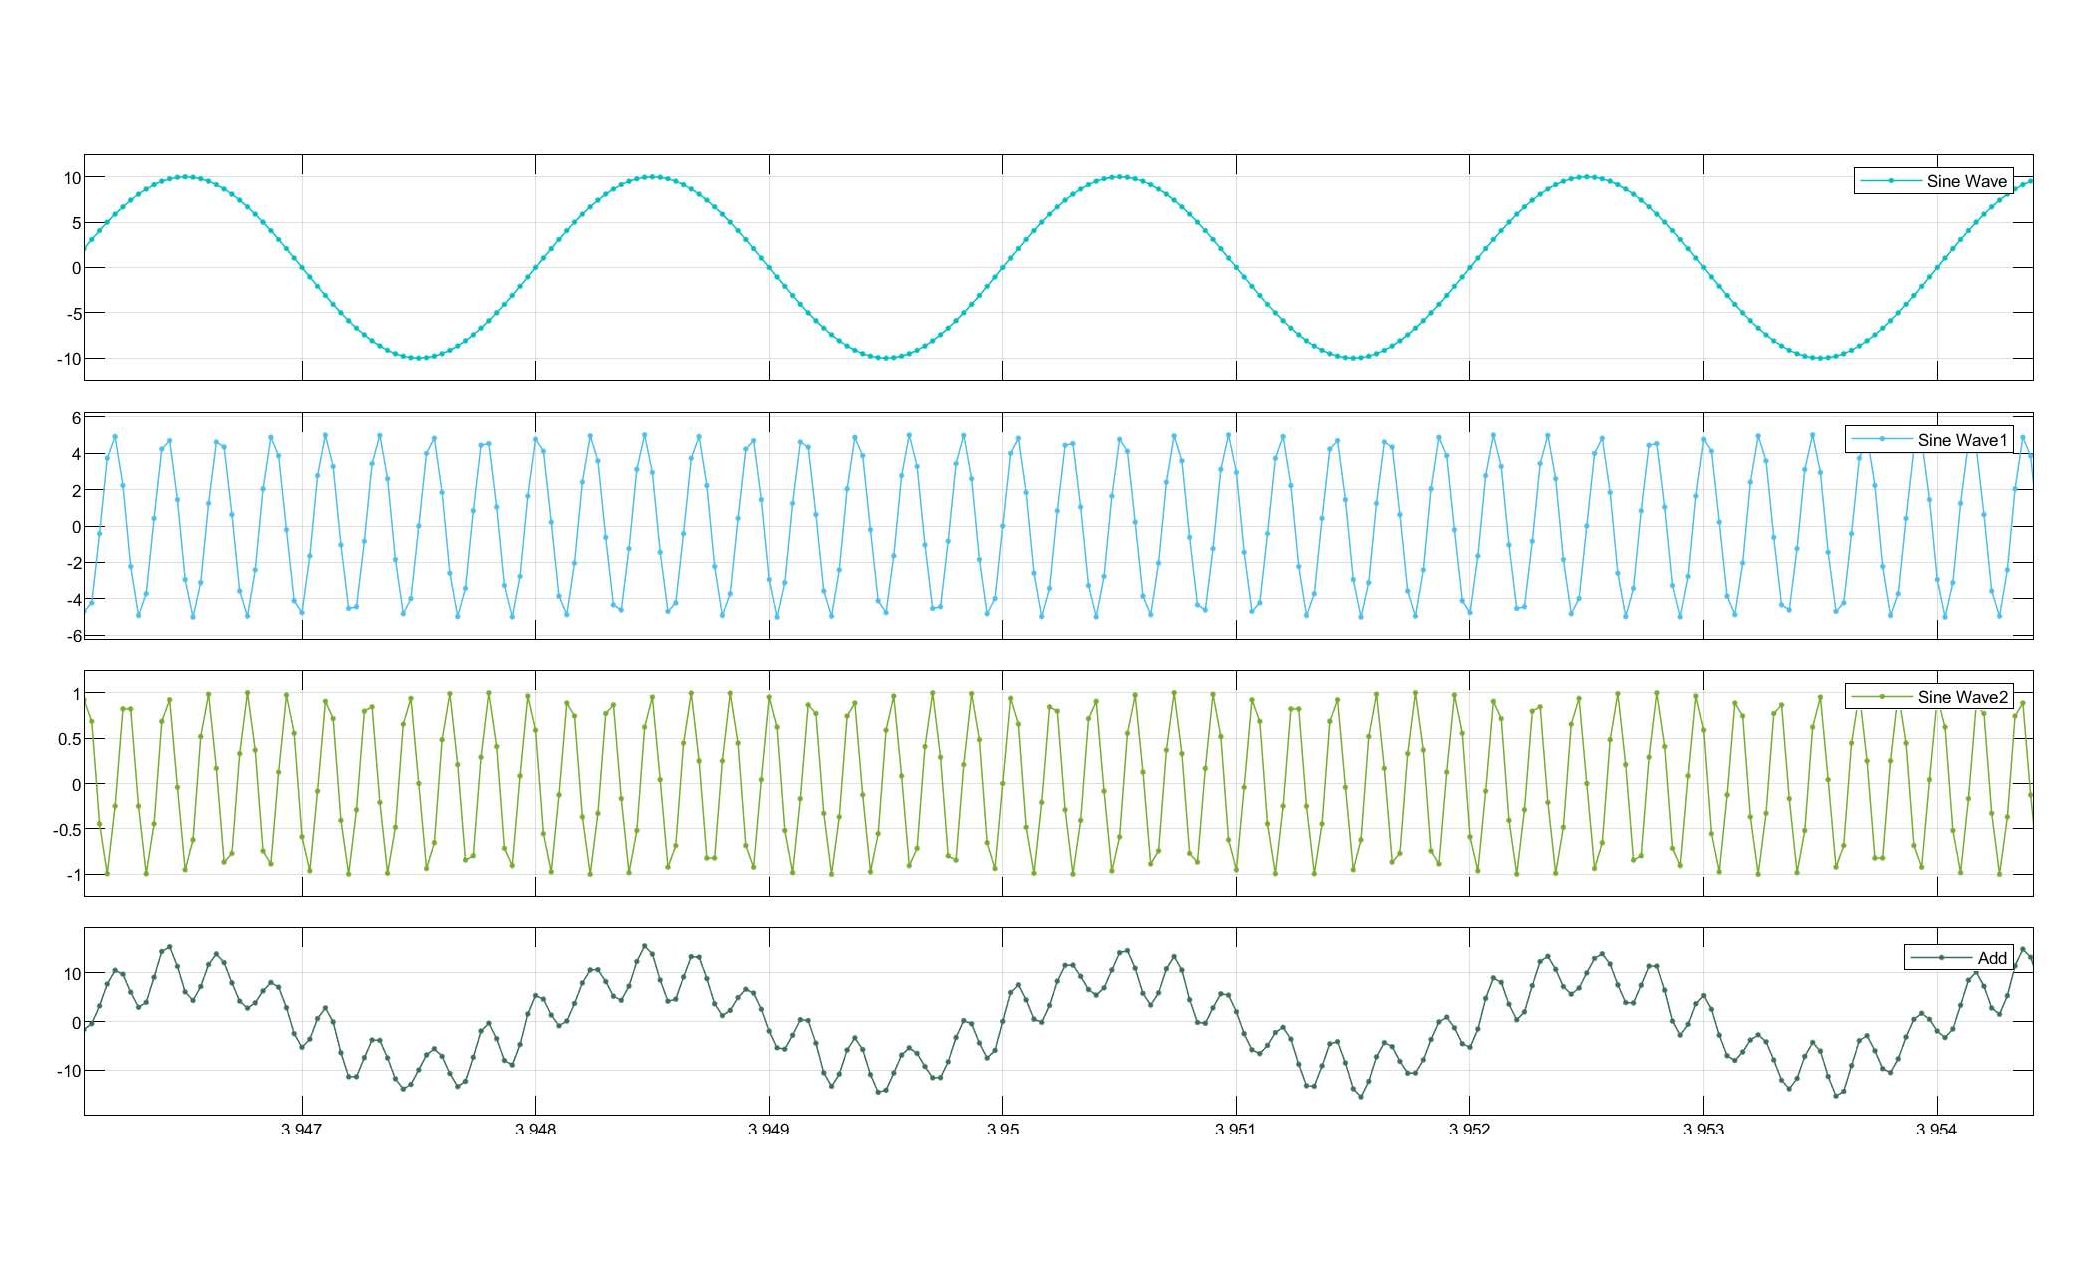
\includegraphics[width=0.95\textwidth]{figure/exp1/sim2_1.pdf}}
    \newline
    \subfloat[采样后的时域波形\label{fig:sim2_2}]{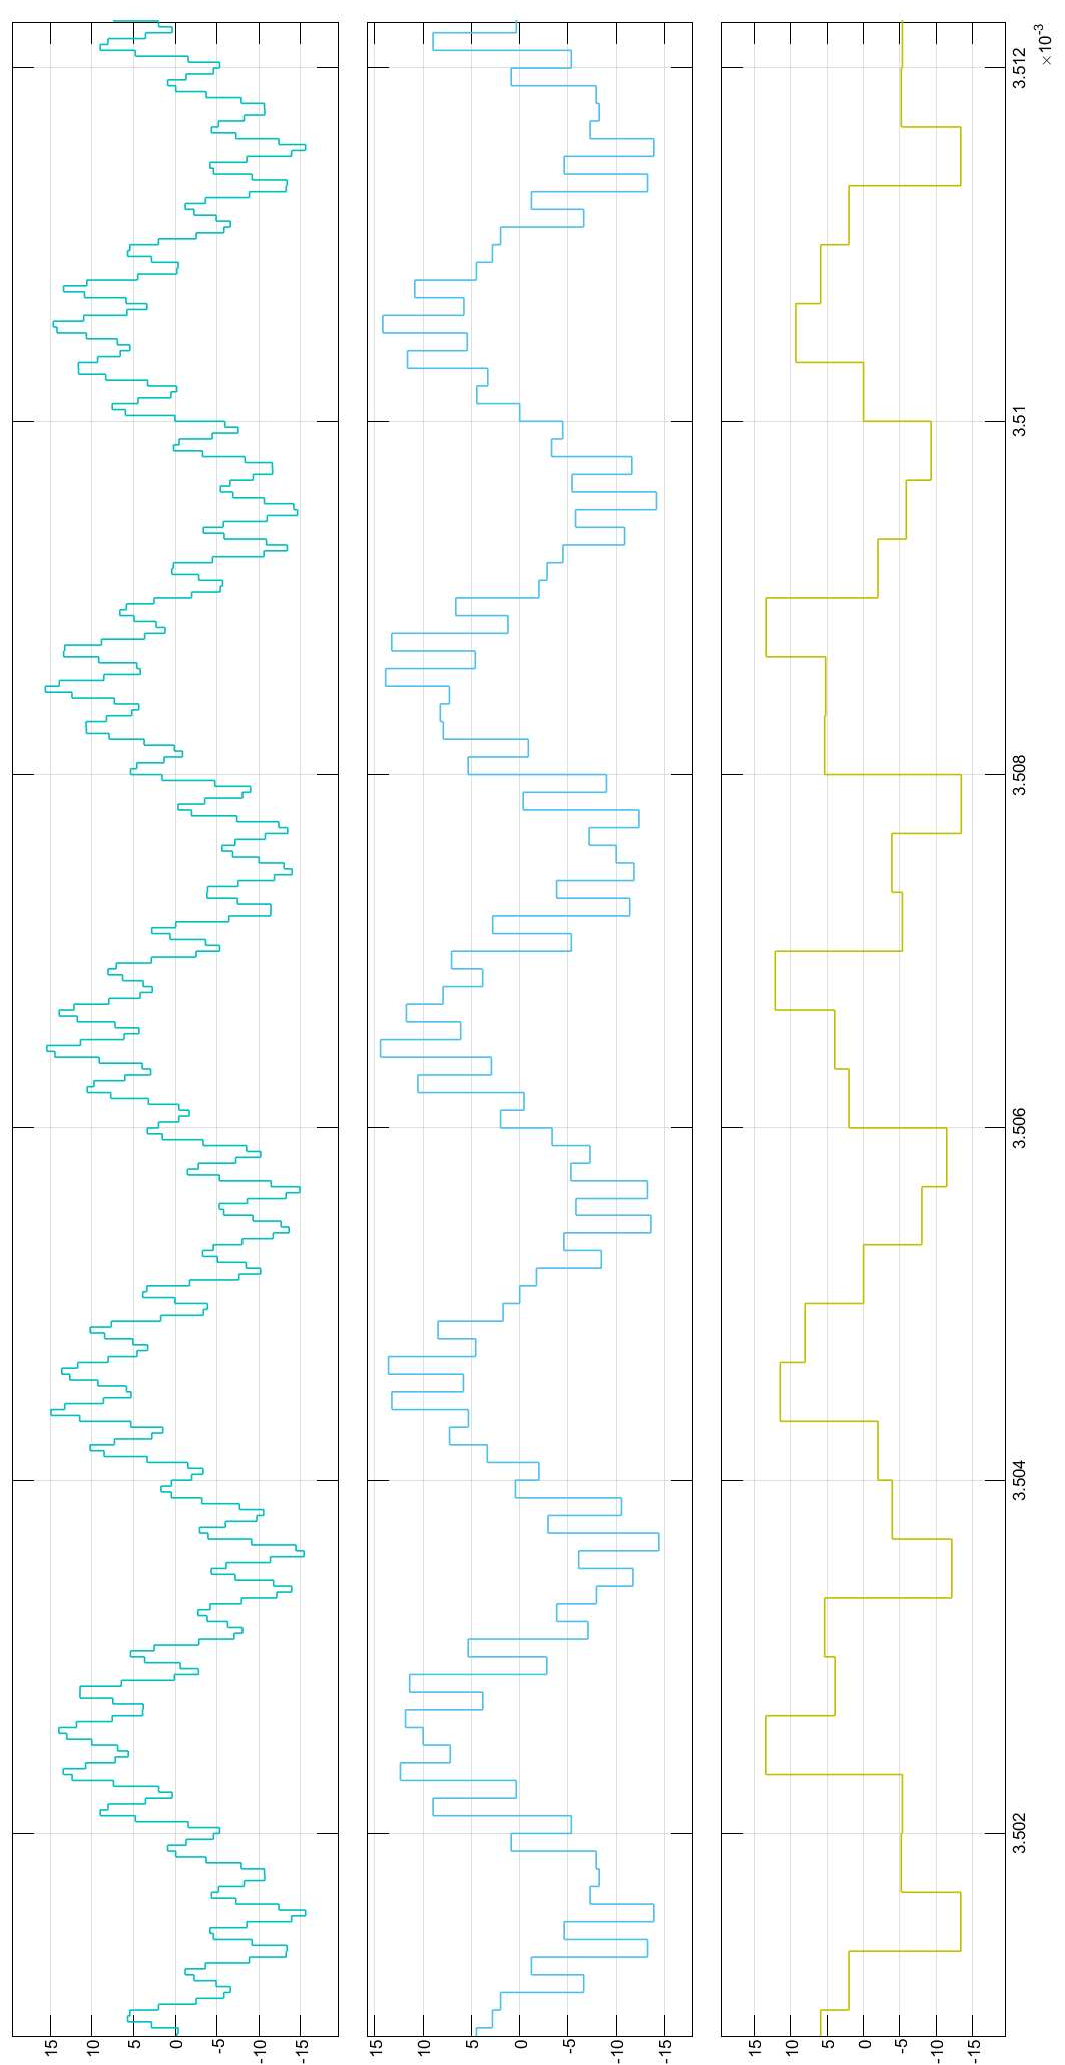
\includegraphics[width=0.47\textwidth,angle=-90]{figure/exp1/sim2_2.pdf}}
    \caption{时域波形仿真结果}
\end{figure}
\begin{figure}[htbp]
  \centering
  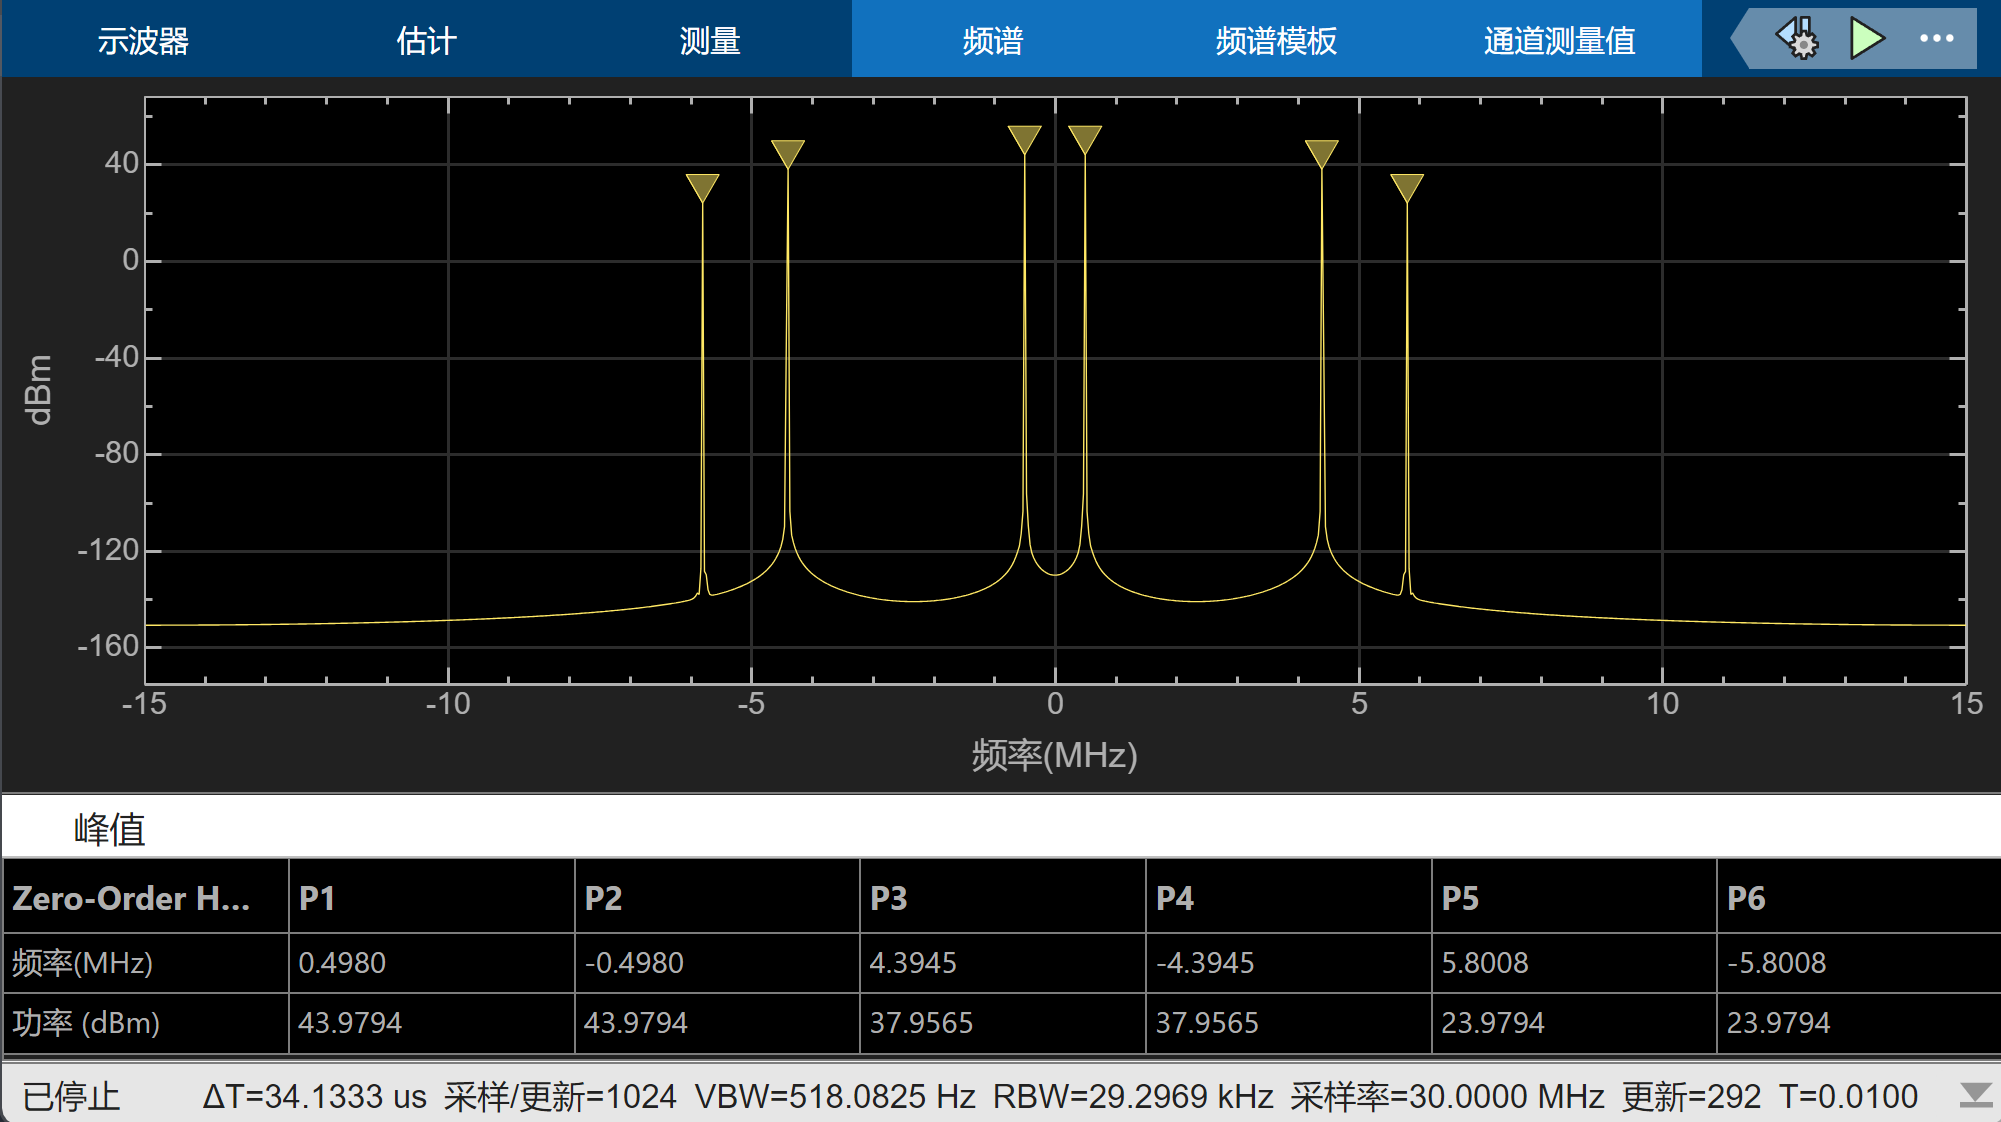
\includegraphics[width=0.75\textwidth]{figure/exp1/30M.png}
  \caption{采样频率为30MHz下的输出频谱}
  \label{fig:spectrum30}
\end{figure}
\begin{figure}[htbp]
  \centering
  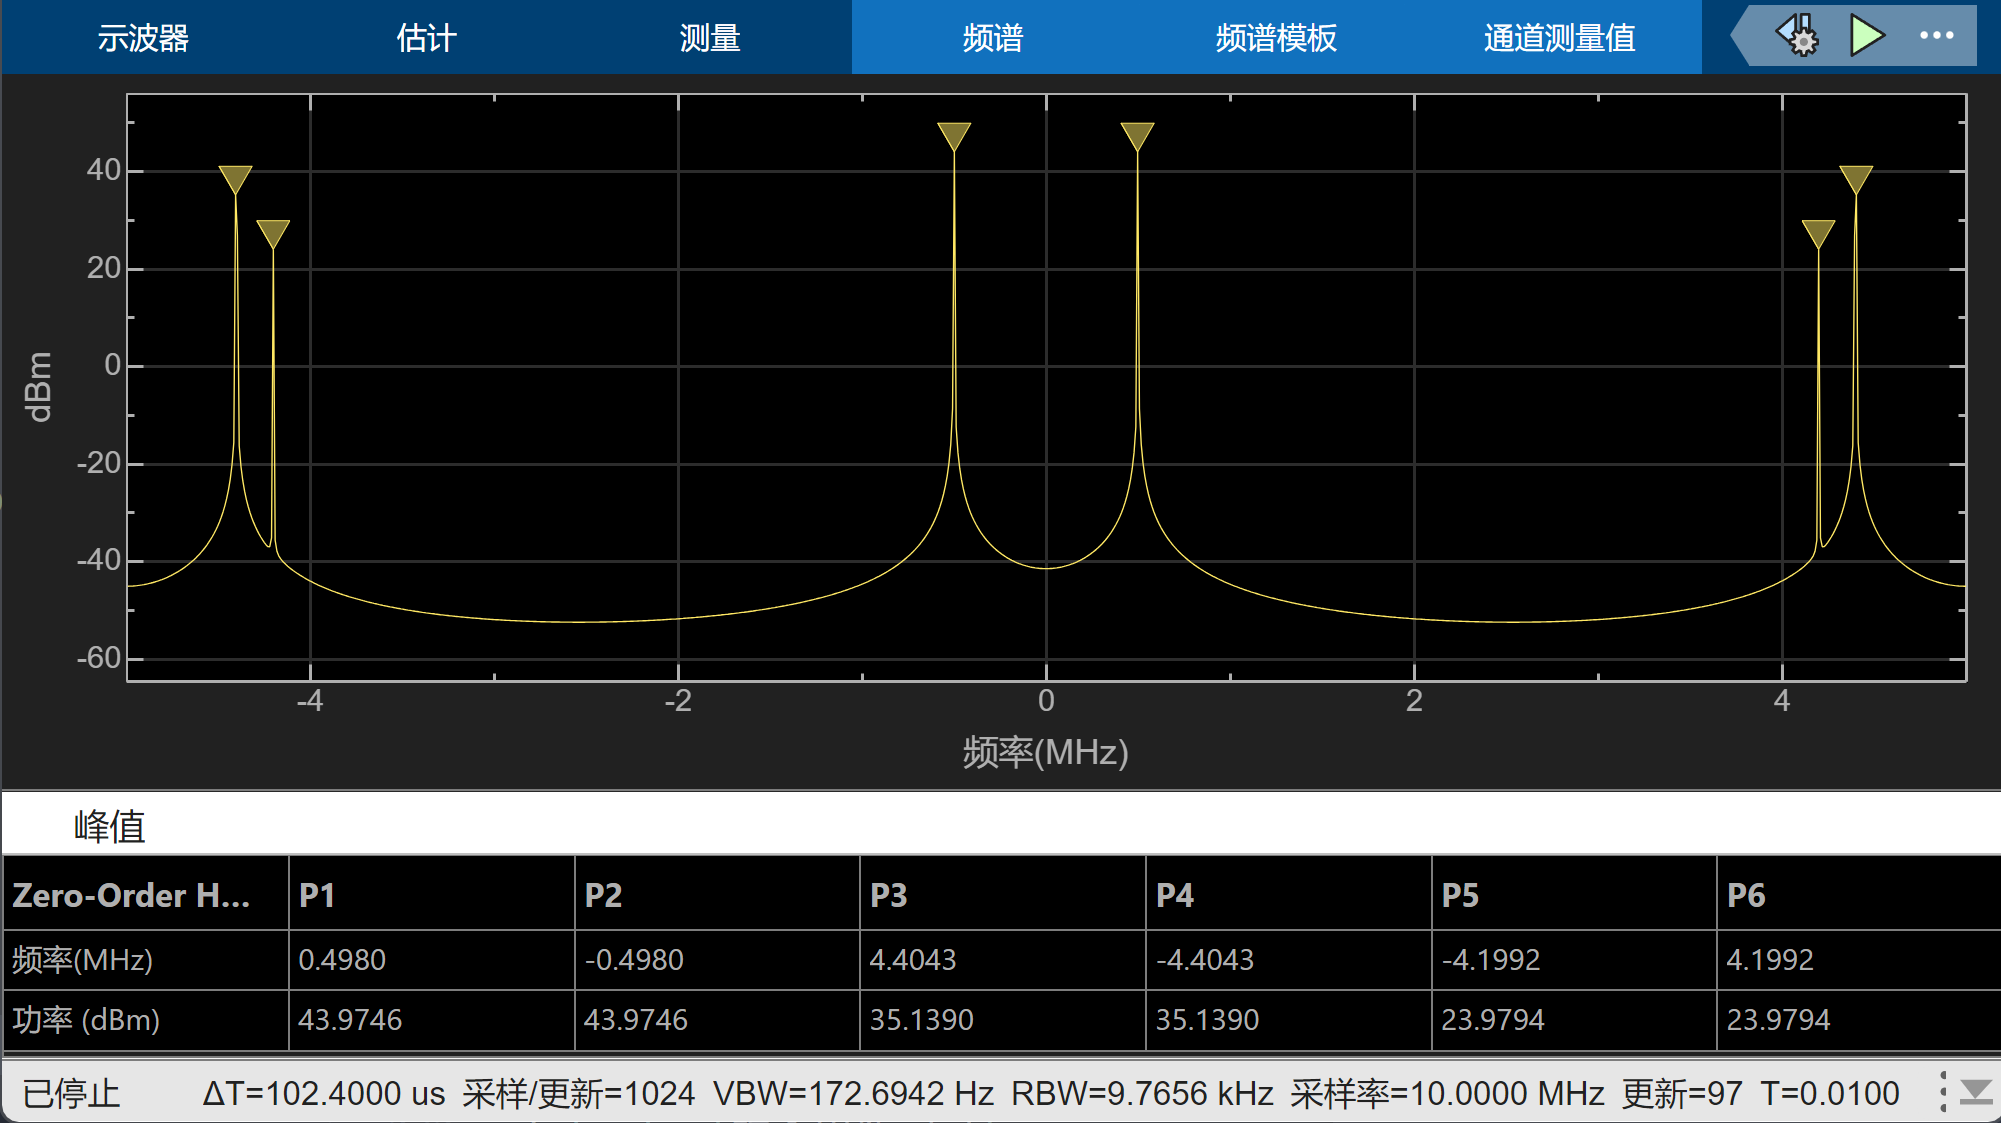
\includegraphics[width=.75\textwidth]{figure/exp1/10M.png}
  \caption{采样频率为10MHz下的输出频谱}
  \label{fig:spectrum10}
\end{figure}
\begin{figure}[htbp]
  \centering
  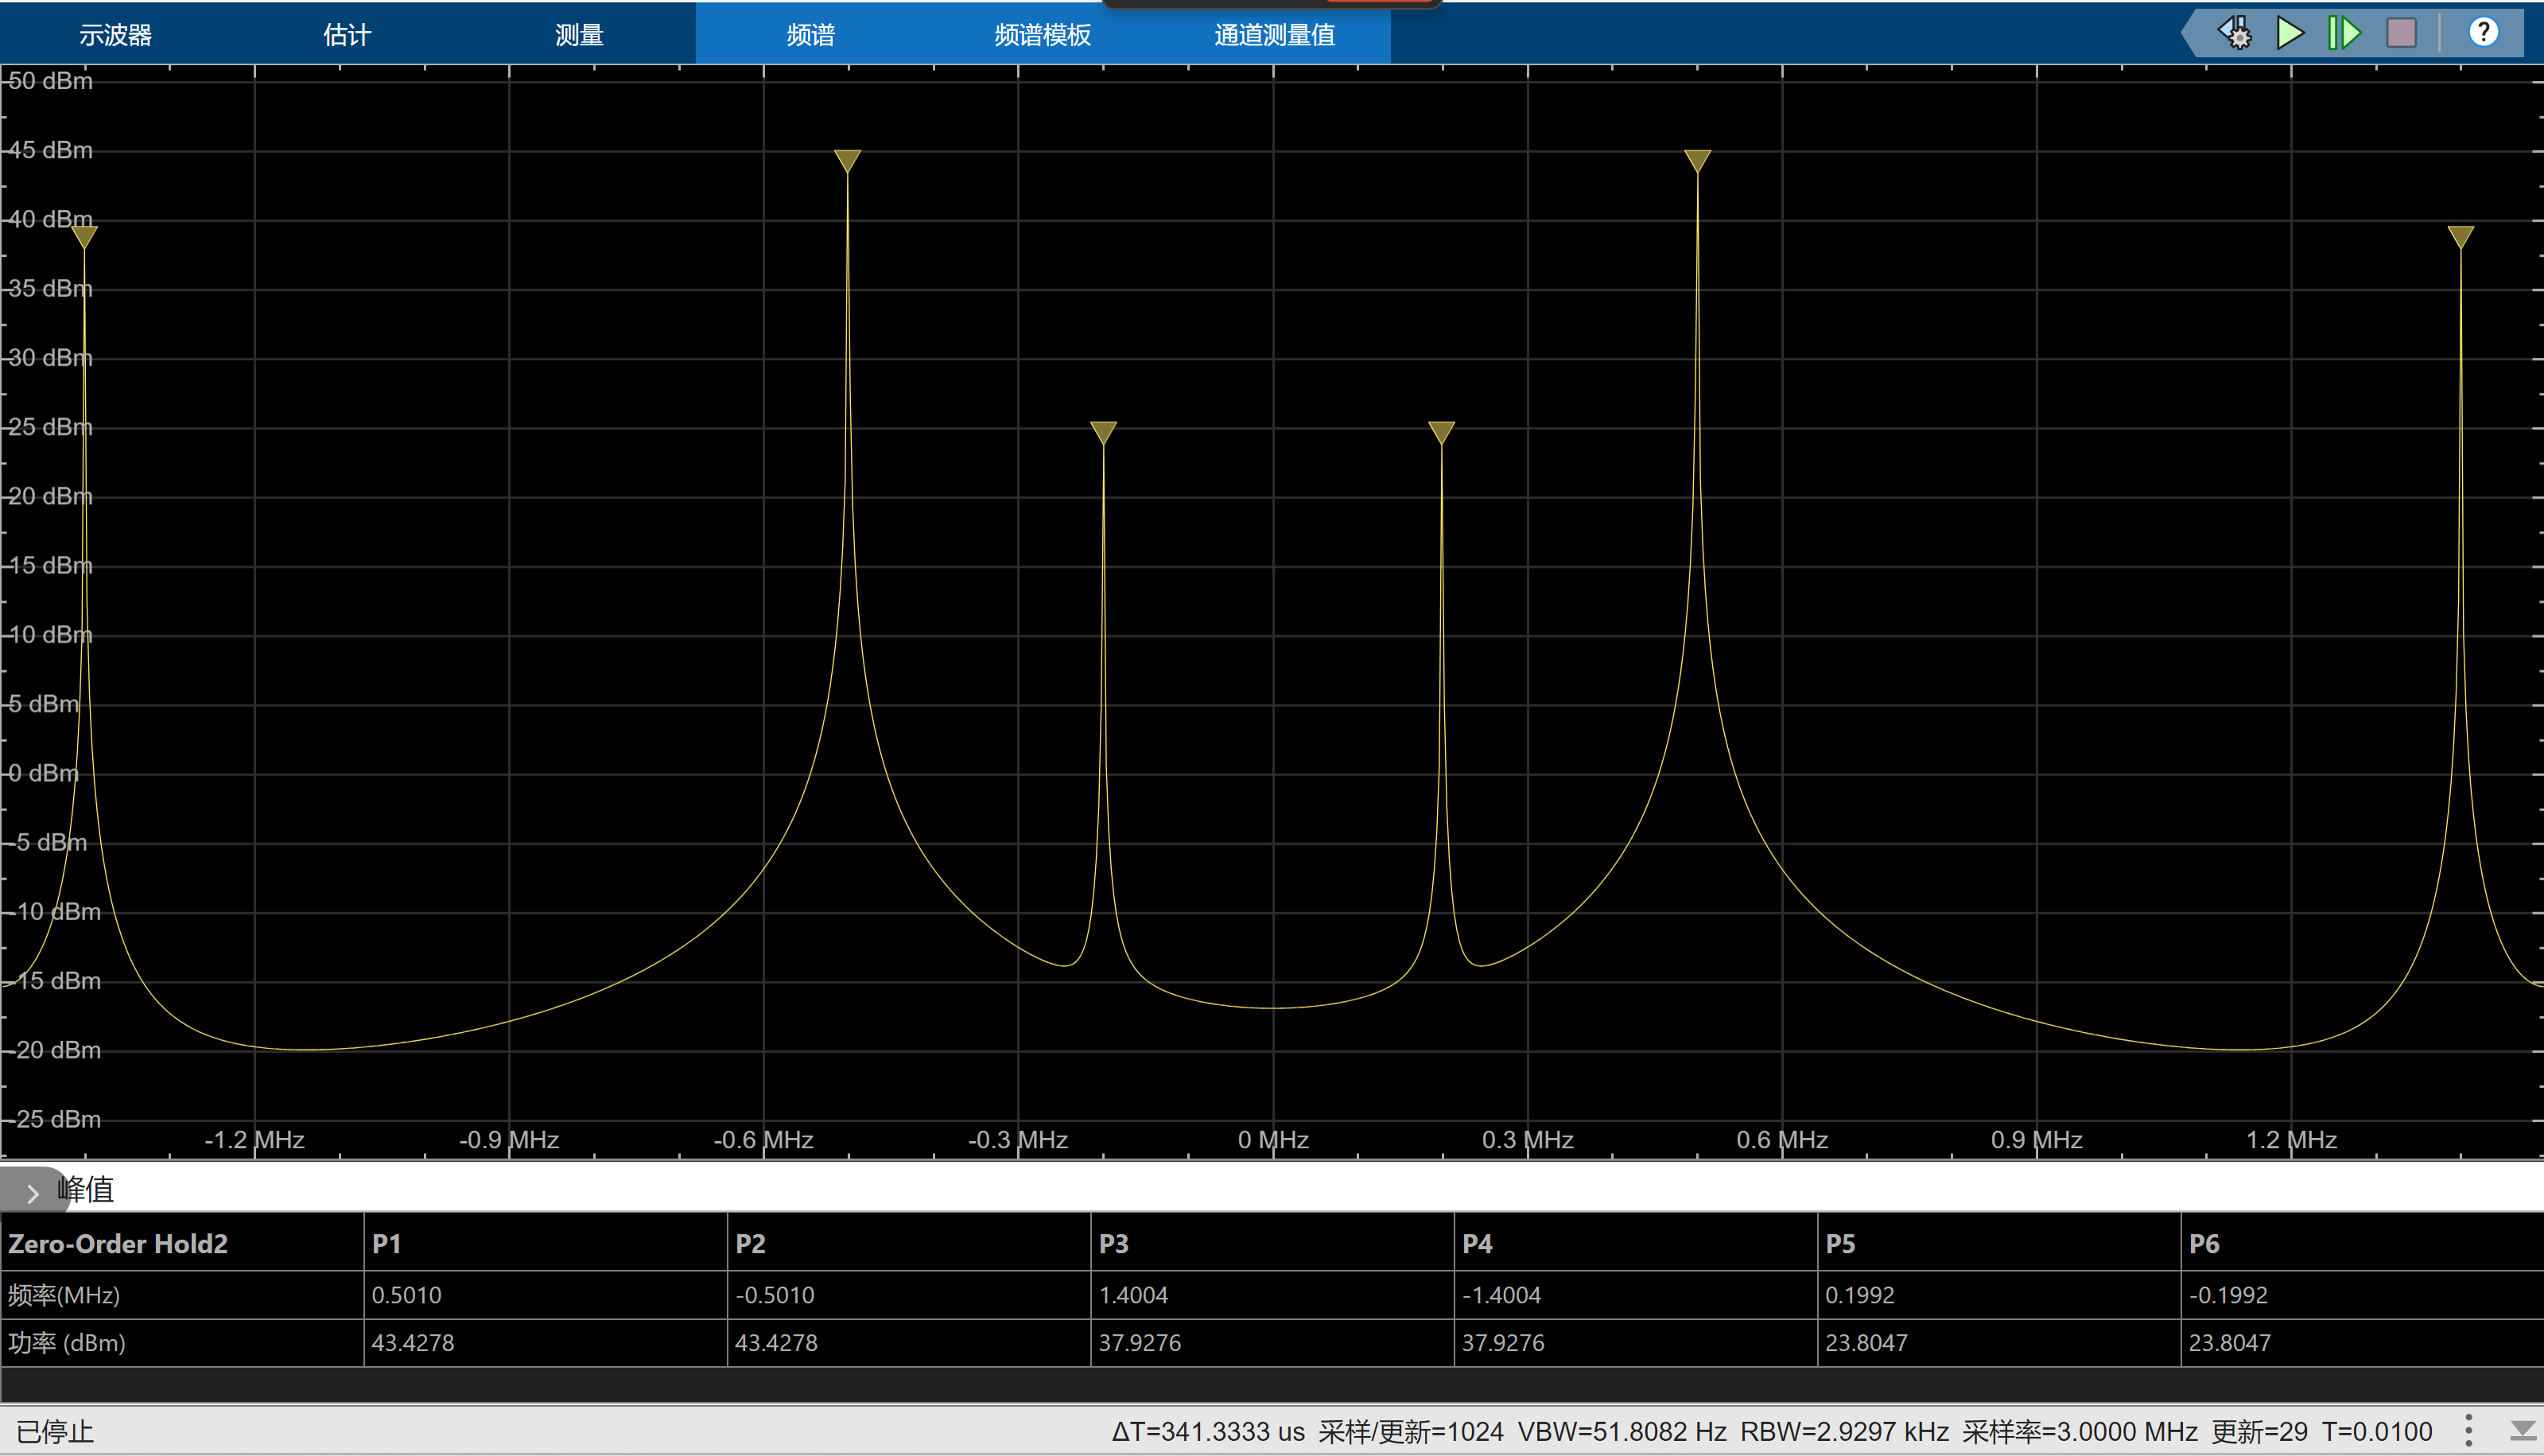
\includegraphics[width=.75\textwidth]{figure/exp1/3M.png}
  \caption{采样频率为3MHz下的输出频谱}
  \label{fig:spectrum3}
\end{figure}
\subsection{基于 MATLAB 的信号采样频谱绘制}
这一部分的实验内容来自《数字信号处理》教材,列举如下。接下来将给出MATLAB代码以及仿真结果。

\begin{example}[一信号是三个正弦信号(频率为50 Hz、500 Hz、1 000 Hz)的和,以8 kHz采样,用适当数量样本画出该信号。]
  \begin{lstlisting}[language=matlab]
fs = 8000; % Sampling frequency, 8 kHz
t = 0:1/fs:1; % Generate time axis, 1 second
f1 = 50;    % First sine wave frequency 50 Hz
f2 = 500;   % Second sine wave frequency 500 Hz
f3 = 1000;  % Third sine wave frequency 1000 Hz

% Signal generation
signal = sin(2*pi*f1*t) + sin(2*pi*f2*t) + sin(2*pi*f3*t);

% Plot time-domain signal
figure;
subplot(2,1,1); % Divide the figure into two parts
plot(t, signal);
title('Time-Domain Signal');
xlabel('Time (seconds)');
ylabel('Amplitude');
grid on;

% Compute and plot spectrum
N = length(signal); % Signal length
fft_signal = fft(signal); % Compute FFT
f = (0:N-1)*(fs/N); % Frequency axis

% Plot only the positive frequency part
half_N = ceil(N/2);
fft_signal = fft_signal(1:half_N);
f = f(1:half_N);

% Compute magnitude spectrum
magnitude = abs(fft_signal)/N;

subplot(2,1,2); % Plot spectrum in the second part of the figure
plot(f, magnitude);
title('Signal Spectrum');
xlabel('Frequency (Hz)');
ylabel('Magnitude');
grid on;

  \end{lstlisting}
\end{example}
仿真结果如图~\ref{fig:fig1}~所示。可以看到频谱在50Hz、500Hz、1000Hz三处分别有一根谱线,这是正弦波的傅里叶变换特性,也证明了频谱分析的意义。
\begin{figure}[htbp]
  \centering
  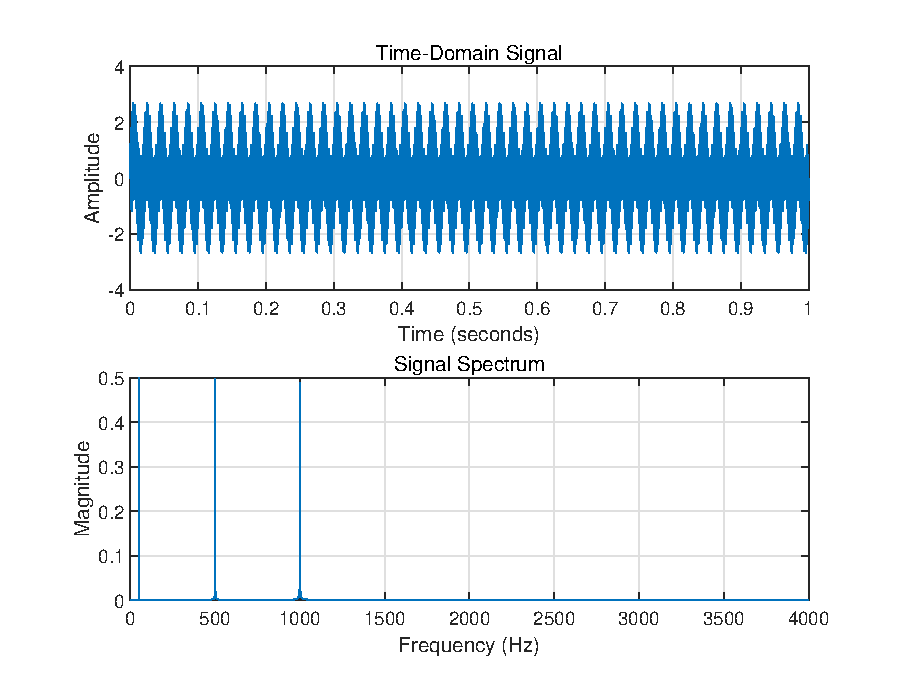
\includegraphics[width=0.65\textwidth]{figure/exp1/fig1.eps}
  \caption{8000Hz采样后的时域频域谱}
  \label{fig:fig1}
\end{figure}
\newpage
\begin{example}[一信号是三个正弦信号(频率为50 Hz、500 Hz、1 000 Hz)的和,以800 Hz采样,用适当数量样本画出该信号,并讨论信号的混叠状况。]
  \begin{lstlisting}[language=matlab]
fs = 800;  % Sampling frequency, 800 Hz
t = 0:1/fs:1; % Generate time axis, 1 second
f1 = 50;    % First sine wave frequency 50 Hz
f2 = 500;   % Second sine wave frequency 500 Hz
f3 = 1000;  % Third sine wave frequency 1000 Hz

% Signal generation
signal = sin(2*pi*f1*t) + sin(2*pi*f2*t) + sin(2*pi*f3*t);

% Plot time-domain signal
figure;
subplot(2,1,1); % Divide the figure into two parts
plot(t, signal);
title('Time-Domain Signal');
xlabel('Time (seconds)');
ylabel('Amplitude');
grid on;

% Compute and plot spectrum
N = length(signal); % Signal length
fft_signal = fft(signal); % Compute FFT
f = (0:N-1)*(fs/N); % Frequency axis

% Compute magnitude spectrum
magnitude = abs(fft_signal)/N;

% Expand frequency range for better visualization
subplot(2,1,2);
plot(f, magnitude);
xlim([0, 1200]); % Set frequency range display from 0 to 1200 Hz
title('Signal Spectrum');
xlabel('Frequency (Hz)');
ylabel('Magnitude');
grid on;

  \end{lstlisting}
\end{example}
仿真结果如图~\ref{fig:fig2}~所示。可以发现,此时的时域谱发生了交叠(闪电型谱线),频域中出现频谱泄露。下面对每条谱线的成因进行分析:
\begin{itemize}
  \item 50Hz:采样前已有频率。
  \item 200Hz:1000Hz频率折叠导致。
  \item 300Hz:500Hz频率折叠导致。
  \item 500Hz:采样前已有频率。
  \item 600Hz:FFT运算带来的1000Hz频率镜像。
  \item 750Hz:50Hz频率折叠。
\end{itemize}
\begin{remark}
该采样不是欠采样,无法重建原有信号。
\end{remark}
\begin{figure}[htbp]
  \centering
  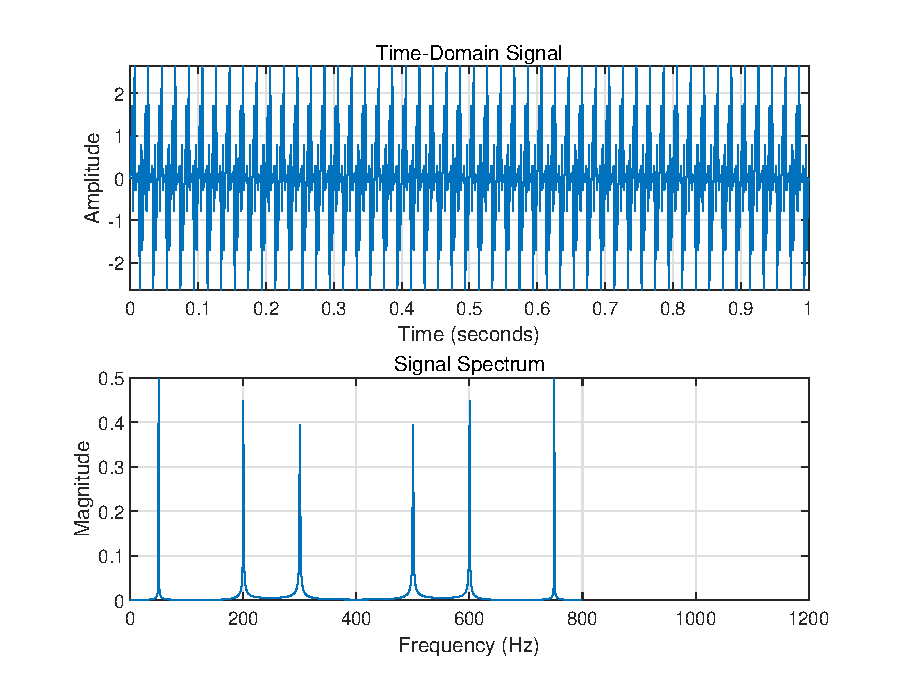
\includegraphics[width=0.65\textwidth]{figure/exp1/fig2.eps}
  \caption{800Hz采样后的时域频域谱}
  \label{fig:fig2}
\end{figure}

\begin{example}[令$x(n) =\cos(2\pi fn/f_s)$,其中$f/f_s$ = 1/16,即每个周期内有16个点。试利用MATLAB编程实现:作M = 4倍的抽取,使每个周期变成4点。作L = 3倍的插值,使每个周期变成48点。
  ]
  \begin{lstlisting}[language=matlab]
f = 1;          % Frequency (Hz)
fs = 16;        % Sampling frequency (Hz)
N = 100;        % Signal length

n = 0:N-1;      % Time sequence
x = cos(2*pi*f*n/fs);  % Original signal

% Perform M = 4 times decimation
M = 4;
x_decimated = decimate(x, M);   % Decimate the signal using the decimate function

% Perform L = 3 times interpolation
L = 3;
x_interpolated = interp(x, L);   % Interpolate the signal using the interp function

% Create a figure to display time-domain and frequency-domain plots
figure;

% First row: Time-domain signals
subplot(3,1,1);
stem(n, x); % Original signal
title('Time-Domain Plot of Original Signal x(n)');
xlabel('Sample index n');
ylabel('Amplitude');
grid on
subplot(3,1,2);
stem(x_decimated);  % Decimated signal
title('Time-Domain Plot of M = 4 Times Decimated Signal');
xlabel('Sample index n');
ylabel('Amplitude');
grid on
subplot(3,1,3);
stem(x_interpolated);  % Interpolated signal
title('Time-Domain Plot of L = 3 Times Interpolated Signal');
xlabel('Sample index n');
ylabel('Amplitude');
grid on
figure;
% Second row: Frequency-domain signals
subplot(3,1,1);
% Spectrum of the original signal
f_orig = abs(fft(x));
f_axis = (0:length(f_orig)-1)*(fs/length(f_orig)); % Frequency axis
stem(f_axis, f_orig);
title('Frequency-Domain Plot of Original Signal x(n)');
xlabel('Frequency (Hz)');
ylabel('Magnitude');
grid on
% Spectrum of the decimated signal
f_dec = abs(fft(x_decimated));
f_axis_dec = (0:length(f_dec)-1)*(fs/M)/length(f_dec); % Frequency axis after decimation

subplot(3,1,2);
stem(f_axis_dec, f_dec);
title('Frequency-Domain Plot of M = 4 Times Decimated Signal');
xlabel('Frequency (Hz)');
ylabel('Magnitude');
grid on
% Spectrum of the interpolated signal
f_interp = abs(fft(x_interpolated));
f_axis_interp = (0:length(f_interp)-1)*(fs*L)/length(f_interp); % Frequency axis after interpolation
subplot(3,1,3);
stem(f_axis_interp, f_interp);
title('Frequency-Domain Plot of L = 3 Times Interpolated Signal');
xlabel('Frequency (Hz)');
ylabel('Magnitude');
grid on
  \end{lstlisting}
\end{example}
仿真结果如图~\ref{fig:fig3}~、~\ref{fig:fig4}~所示,经检验发现符合题目要求。
\begin{figure}[htbp]
  \centering
  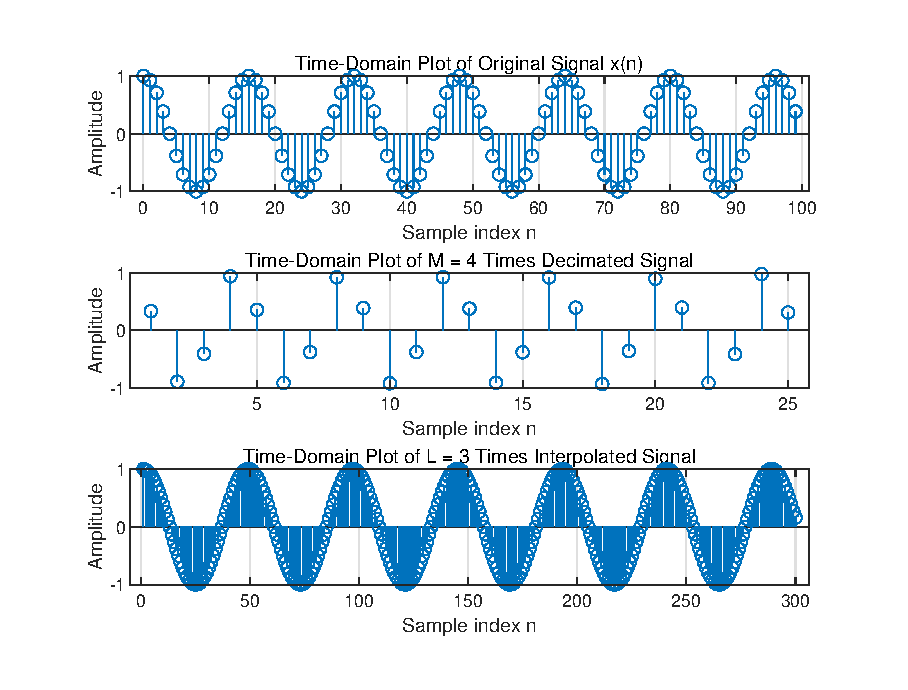
\includegraphics[width=0.65\textwidth]{figure/exp1/fig3.eps}
  \caption{原信号,$M=4$抽取,$L=3$内插后的时域谱}
  \label{fig:fig3}
\end{figure}
\begin{figure}[htbp]
  \centering
  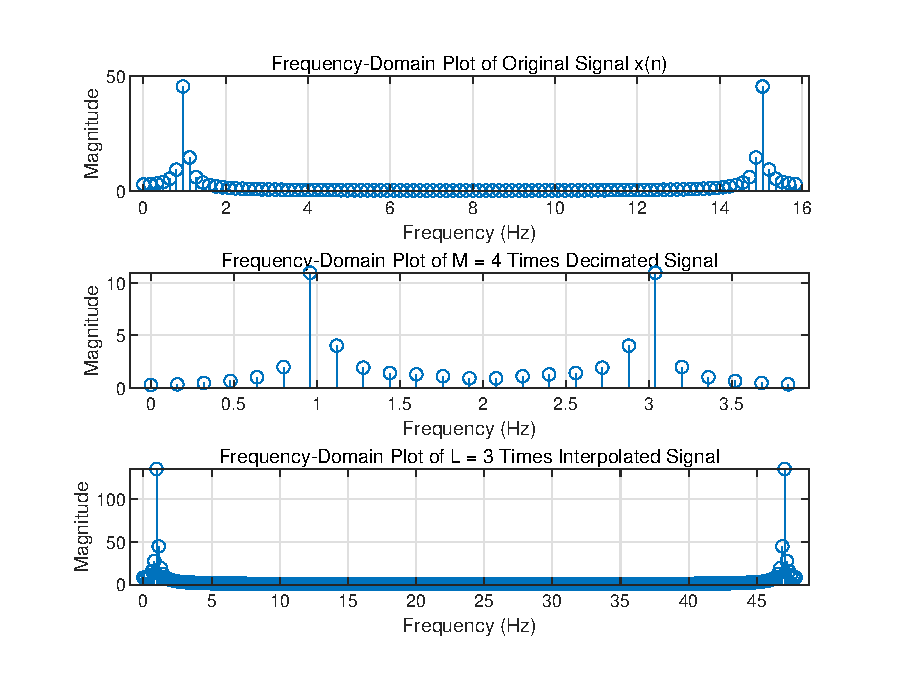
\includegraphics[width=0.65\textwidth]{figure/exp1/fig4.eps}
  \caption{原信号,$M=4$抽取,$L=3$内插后的频域谱}
  \label{fig:fig4}
\end{figure}
\begin{example}[输入信号$x(n)$为归一化频率分别是$f_1$ = 0.04,$f_2$= 0.3的正弦信号相加而成,$N$ = 50,内插因子$L$为5,抽取因子$M$为3,给出按有理因子5/3作采样率转换的输入输出波形。]
  \begin{lstlisting}[language=matlab]
f1 = 0.04;        % Normalized frequency f1
f2 = 0.3;         % Normalized frequency f2
N = 50;           % Signal length

n = 0:N-1;        % Time sequence
x1 = sin(2*pi*f1*n);  % First sine wave
x2 = sin(2*pi*f2*n);  % Second sine wave

% Generate the input signal
x = x1 + x2;

% Set interpolation and decimation factors
L = 5;    % Interpolation factor
M = 3;    % Decimation factor

% Perform sampling rate conversion with a rational factor of 5/3
x_resampled = resample(x, L, M);  % Use the resample function

% Create a figure to display time-domain and frequency-domain plots
figure;

% First row: Time-domain signals
subplot(2,1,1);
stem(n, x); % Input signal
title('Original Signal');
xlabel('n');
ylabel('Amplitude');
grid on
subplot(2,1,2);
stem(x_resampled);  % Resampled signal
title('Resampled Signal');
xlabel('n');
ylabel('Amplitude');
grid on
figure;
% Second row: Frequency-domain signals
subplot(2,1,1);
% Spectrum of the input signal
f_orig = abs(fft(x));
f_axis = (0:length(f_orig)-1)*(1/N); % Normalized frequency
stem(f_axis, f_orig);
title('Frequency Characteristics of Original Signal');
xlabel('Frequency (Hz)');
ylabel('Magnitude');
grid on
subplot(2,1,2);
% Spectrum of the resampled signal
f_resampled = abs(fft(x_resampled));
f_axis_resampled = (0:length(f_resampled)-1)*(1/length(x_resampled)); % Normalized frequency
stem(f_axis_resampled, f_resampled);
title('Frequency Characteristics of Resampled Signal');
xlabel('Frequency (Hz)');
ylabel('Magnitude');
grid on
  \end{lstlisting}
\end{example}
仿真结果如图~\ref{fig:fig5}~、~\ref{fig:fig6}~所示。经检验发现符合题目要求。
\begin{figure}[htbp]
  \centering
  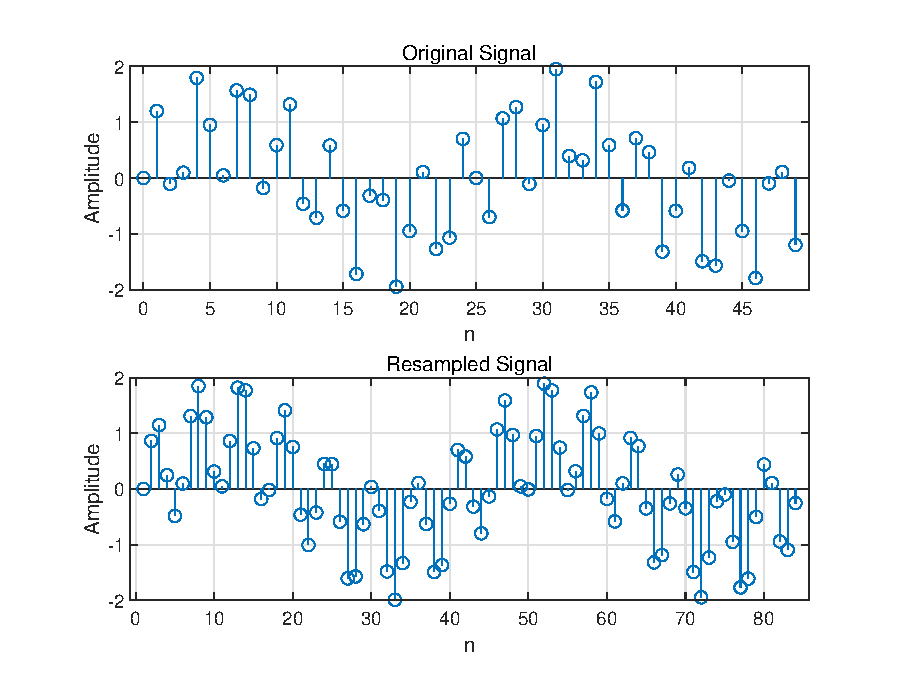
\includegraphics[width=0.65\textwidth]{figure/exp1/fig5.eps}
  \caption{5/3采样率转换后的时域谱}
  \label{fig:fig5}
\end{figure}

\begin{figure}[htbp]
  \centering
  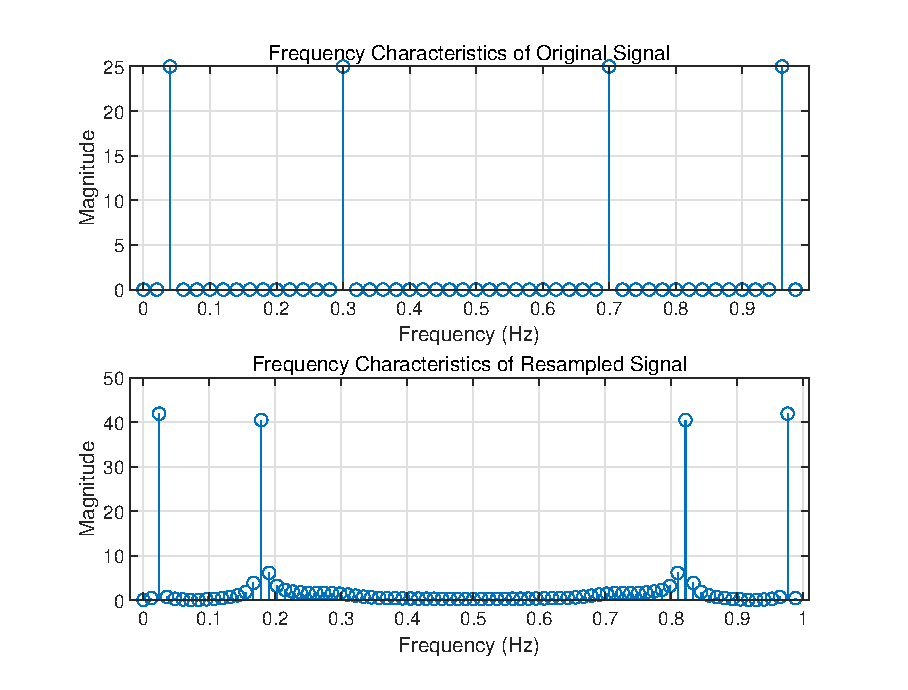
\includegraphics[width=0.65\textwidth]{figure/exp1/fig6.eps}
  \caption{5/3采样率转换后的频域谱}
  \label{fig:fig6}
\end{figure}